\section{GPU Architecture Trends}

It is impossible to predict what the future of GPUs would be. However, by
examining the history and current state of GPU architectures, we might be able
to identify some trends. Knowing these trends are essential to software
designers so that they can plan ahead and design softwares that not only work
efficiently on currently available architectures, could potentially work
well on future ones. Furthermore, sometimes an architectural trend reveals a
growing need for some software-side considerations, which could be taken into
account in the form of a programming practice, a compiler optimization, or a
runtime software layer.

\begin{figure}[t]
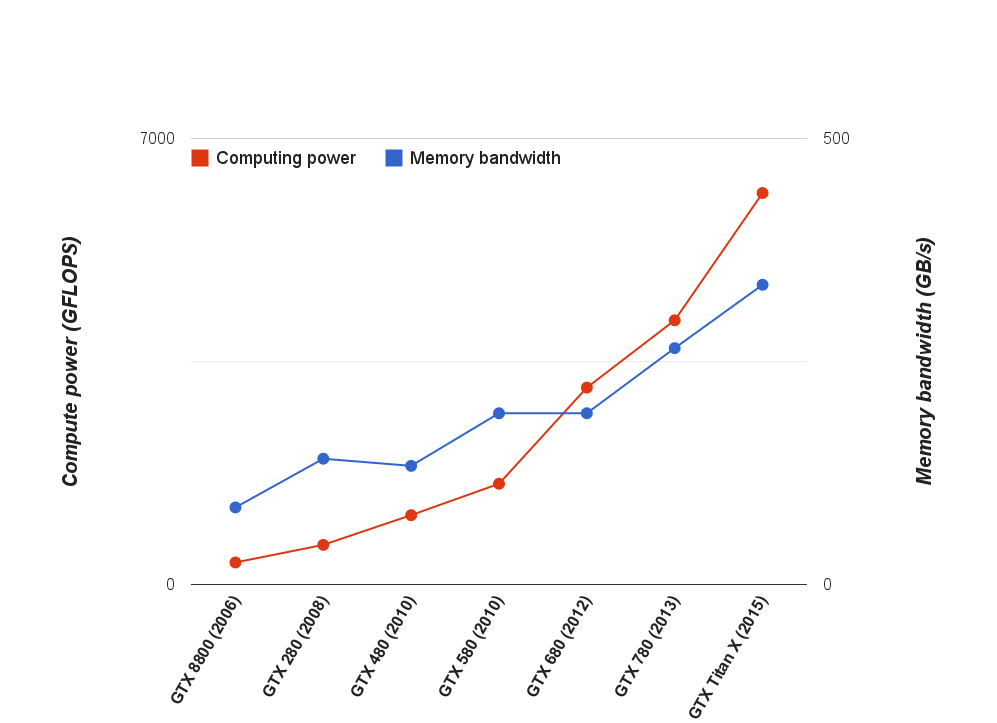
\includegraphics[scale=0.5]{computevsmemory.png}
\caption{Computing power vs. memory bandwidth.}
\label{fig:computevsmemory}
\end{figure}



Figure~\ref{fig:computevsmemory} illustrates the increase in computing power
(GFLOPS) and memory bandwidth (GB/s) of NVIDIA GPUs from their earliest
CUDA-enabled version to date. As can be seen, GPU computing power has been
increasing steadily with a positive slope. On the other hand, even though GPU
memory bandwidth is also increasing, it appears that it is falling behind. In
other words, the GPUs offered byte per FLOPS is gradually decreasing -- from
250 bytes/FLOPS in GTX 8800 to 41 bytes/FLOP in GTX 880. If this trend
continues, as we go forward, more and more GPU applications will be bound by
the memory performance. In such applications, GPU threads would be mostly idle
waiting for the data to be accessed from memory. As a result, the approach to
optimize the GPU applications for memory hierarchy will become more and more
attractive. Consequently, therefore, some applications might even decide on
sacrificing GPU computing power in return for a better memory performance (e.g.
executing extra instructions to re-layout the data for more efficient memory
accesses)~\cite{}.


\begin{figure}[t]
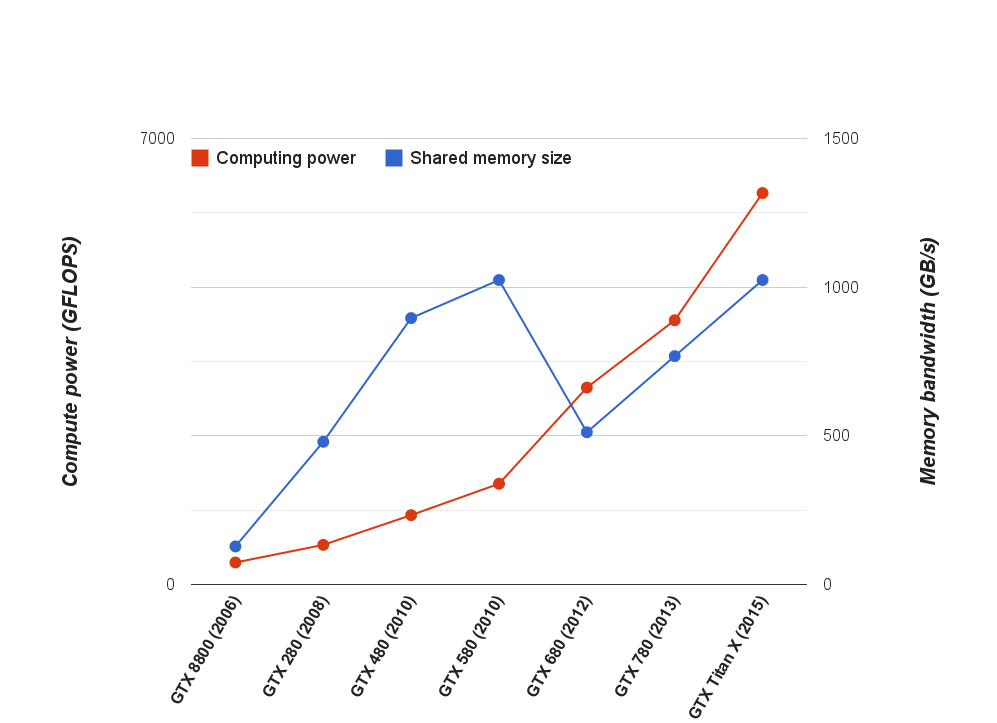
\includegraphics[scale=0.5]{computevsshared.png}
\caption{Computing power vs. shared memory size.}
\label{fig:computevsshared}
\end{figure}

Figure~\ref{fig:computevsshared} shows the changes in the total size of on-chip
memory (L1 cache + shared memory) available in the same set of GPUs. Although a
very clear increasing or decreasing trend for the size of on-chip memory in
progressive generations of GPUs is not observable from this graph, two implicit
findings can be extracted from it. First, considering the steady increase in
the GPU computing power, the available size of on-chip memory does not seem to
be scaling well enough to a point where it can potentially host a non-thrashing
L1 cache.

Second, due to the non-constant changes in the available size of shared memory
from architecture generation to generation, GPU programmers cannot not rely on
a static size of on-chip memory in their applications. Ideally, instead, one
needs to design GPU applications so that they automatically configure
themselves at runtime given the available size of on-chip memory available on
the running GPUs (which might be different from run to run). Such
configurations include the proper size of shared memory to use by each
thread/thread-block and also the size and formation of GPU threads.

